\documentclass[11pt]{article}
\usepackage{times}
\usepackage{verbatim}
\usepackage[pdftex]{graphicx}    
\usepackage[pdftex]{color}  
\usepackage{fullpage}
\usepackage{url}
\usepackage{cite}

\bibliographystyle{plos}

% \draftfalse: submission version. Legends,tables at end. No figs included.
% \drafttrue:   online preprint. Figures and table inline.
\newif\ifdraft
%\draftfalse
\drafttrue

\renewcommand{\baselinestretch}{1.5}
\setcounter{secnumdepth}{0}


\begin{document}

\title{Infernal 1.0: inference of RNA alignments}
\author{Eric P. Nawrocki and Sean R. Eddy\\
HHMI Janelia Farm Research Campus\\
19700 Helix Drive\\
Ashburn VA 20147\\
\url{http://selab.janelia.org/}\\
}
%\date{\today}
\maketitle


%%%%%%%%%%%%%%%%%%%%%%%%%%%%%%%%%%%%%%%%%%%%%%%%%%%%%%%%%%%%%%%%%%%%%%

\section{Introduction}

\begin{comment}
\textsc{infernal} is a software package for building consensus RNA
secondary structure profiles called \emph{covariance models} (CMs),
and using them to search nucleic acid sequence databases for
homologous RNAs, or to create new sequence and structure-based
multiple sequence alignments. 
\end{comment}

RNAs conserve sequence and structural features that are important for their
function.  When computationally searching for homologous RNAs in
genomic sequence it is beneficial to score both types of conservation.
There have been several tools developed based on this premise.  These
include programs for finding members of one particular family, such as
tRNAs \cite{LoweEddy97,Laslett04}, snoRNAs
\cite{LoweEddy99,Schattner06}, microRNAs \cite{Lai03,Lim03} and SRP
RNAs \cite{Lai03,Lim03}, as well as pattern matching approaches that
require expertly designed query patterns \cite{Macke01}. The most
generally useful tools, however, take as input any RNA (or RNA
multiple alignment) and construct an appropriate scoring system for
scanning and ranking putative homologs within a target database
\cite{Gautheret01,ZhangBafna05}. We describe an implementation of this
general approach in the sofware package \textsc{infernal}.
\textsc{infernal} builds consensus RNA secondary structure profiles
called \emph{covariance models} (CMs), and uses them to search nucleic
acid sequence databases for homologous RNAs, or to create new sequence
and structure-based multiple sequence alignments.  \textsc{infernal}
is used to help annotate RNAs in genomes in conjunction with the
\textsc{Rfam} database \cite{Griffiths-Jones05}, which contains 603
RNA families, each represented by a structural alignment and a CM.

CMs are profile probabilistic models that model both the conserved
primary sequence and well-nested secondary structure of an RNA family.
(CMs are unable to model pseudoknotted structures or other
non-well-nested tertiary structural contacts). A CM is built from a
multiple sequence alignment with consensus structure annotation
denoting which positions of the alignment are single stranded and
which are base paired. CMs have position specific scores for all
possible residues at single stranded positions and all possible base
pairs at paired positions, as well as position specific scores for
insertions and deletions. These scores are derived from the observed
counts of residues, base-pairs, inserts and deletions in the input
alignment, augmented with prior information derived from large
structural ribosomal RNA alignments. The construction and
parameterization of CMs has been described in more detail elsewhere
\cite{Eddy94,infguide03,Eddy02b,NawrockiEddy07}.

\section{Usage} 
\textsc{infernal} is composed of several programs that are used in
combination to build models, search databases, and align putative
homologs by following four basic steps:

\begin{enumerate}
\item Build a covariance model file from a training alignment.

The \emph{cmbuild} program takes as input a structural multiple
RNA alignment in Stockholm format \cite{infguide03} and creates a CM
file that is used by other \textsc{infernal} programs.

\item Calibrate the CM file for similarity search.

Prior to searching databases, approximate E-value statistics for a CM
are estimated using the \emph{cmcalibrate} program. This step is
optional and computationally expensive (as shown in Table 2), but is
required to obtain E-values that estimate the statistical significance
of each hit during similarity search. \emph{cmcalibrate} will also
determine appropriate HMM filter thresholds to use to accelerate
searches without an appreciable loss of sensitivity.

\item Search databases for putative homologs.

The \emph{cmsearch} program reads a model from a CM file and searches
a sequence file for high scoring hits to the model. The output of
\emph{cmsearch} includes an alignment of each hit in a BLAST-like
format augmented with structure annotation.  

\item Align putative homologs to the model.

\emph{cmalign} takes as input a CM file and a target sequence file 
containing putative homologs and aligns the full length sequences to
the model, creating a structurally annotated multiple alignment in
Stockholm format.

\end{enumerate}

Some of these steps are unnecessary for some applications. For
example, a user that wants to only generate alignments of previously
defined homologous sequences, such as small subunit ribosomal RNA
sequences (SSU rRNA), would skip the calibration and search steps. 

For similarity search applications, where the goal is to identify new
examples of a family, it is reasonable to repeat these four steps
multiple times.  Finding new homologs in the search step, adding them
to the training alignment in the alignment step, and building a new
model from the expanded training alignment in the build step of a new
iteration, and so on.

\section{Performance}
An independent benchmark found that \textsc{infernal} and other CM
based methods are the most sensitive and specific available tools for
structural RNA homology search \cite{Freyhult07}.  We have previously
published our own \textsc{Rfam} based benchmark that supports this
\cite{NawrockiEddy07}. Here, we have updated this benchmark to make it
more realistic as described in \emph{Methods}. The results in Figure 1
in the form of an ROC curve show that for this benchmark
\textsc{infernal} 1.0 is significantly more specific and sensitive
than a previous version (0.72) and \textsc{BLAST} family pairwise
search.  

The increased sensitivity comes at a huge cost in compute time
relative to \textsc{BLAST} because CM search algorithms are
computationally expensive. To address this, \textsc{infernal} 1.0
estimates when it is possible to use HMM filters to accelerate search
without sacrificing appreciable sensitivity, and automatically employs
them in such cases. (This automatic HMM filter use only applies to CM
files that have been calibrated with \emph{cmcalibrate}).  The HMMs
used are a reimplementation of the maximum likelihood HMMs developed
by Weinberg and Ruzzo \cite{WeinbergRuzzo06}.  The performance of
\textsc{infernal} with and without filters is shown in Figure 1. The
filters accelerate similarity search for the benchmark by about
13-fold overall, while sacrificing a small amount of sensitivity.
This is a partial, but not complete solution to the problem, as
\textsc{BLAST} is still more than three orders of magnitude faster
than \textsc{infernal}. Table 1 shows running times for similarity
search for six RNA families of various sizes with and without
filters. The range of speedups from filters vary widely. In general,
the more primary sequence conservation in a family, the more effective
an HMM filter will be, although this is not always the case. Further
acceleration remains a major goal of \textsc{infernal} development.

%%%%%%%%%%%%%%%%%%%%%%%%%%%%%%%%%
\begin{comment}
For the problem of structural RNA alignment, no benchmarks of profile
based methods have been published so it is impossible to comment on
alignment accuracy. 
\end{comment}
%%%%%%%%%%%%%%%%%%%%%%%%%%%%%%%%%

The computational cost of CM alignment with the \emph{cmalign} program
has been a limitation of previous versions of
\textsc{infernal}. Version 1.0 uses a constrained dynamic programming
approach first developed by Michael Brown \cite{Brown00} that uses
sequence specific bands derived from a first-pass HMM alignment. This
technique offers a dramatic speedup relative to unconstrained
alignment, especially for large RNAs such as small and large subunit
(SSU and LSU) ribosomal RNAs, which can now be aligned in roughly 1
and 3 seconds per sequence, respectively (Table 1), as opposed to 12
minutes and three hours in previous versions (data not shown).

%%%%%%%%%%%%%%%%%%%%%%%%%%%%%%%%%
\begin{comment}
\textsc{infernal} can
optionally annotate output alignments with posterior probabilities,
which are ``confidence estimates'' that each residue of the alignment
is correctly aligned \cite{Durbin98}.
\end{comment}
%%%%%%%%%%%%%%%%%%%%%%%%%%%%%%%%%

\section{Limitations}
The \emph{cmbuild} program requires as input a structurally annotated
multiple sequence alignment to build a CM. \textsc{infernal}
\emph{cannot} be used to create such alignments by predicting the
structure of an existing alignment, or by inferring a structural
alignment from unaligned sequences \emph{de novo}. (\emph{Should we
add here a list of programs that can create structural
alignments?}). Due to the high computational complexity of CM
algorithms, \textsc{infernal} is compute intensive and using it for
homology search in large databases requires a large cluster (see
timings in Table 1).

\section{Methods}
Briefly, the updated \textsc{Rfam} benchmark corresponding to Figure 1
was constructed as follows. The sequences of the seed alignments of
503 Rfam (release 7) families were clustered based on sequence
identity given the alignment using single linkage clustering. Families
for which two clusters A and B existed such that no sequence in
cluster A is more than 60\% identical to a sequence in cluster B and
the larger of A and B had at least five sequences were selected for
the benchmark. The larger of the clusters was defined as a training
set, the smaller as a test set. Fifty-one such families meet these
criteria, yielding 450 test sequences. (These are the same 51 families
and 450 test sequences from the benchmark in
\cite{NawrockiEddy07}). To simulate a homology search exercise in
realistic genomic sequence, the test sequences were randomly embedded
in a 1 Mb pseudogenome that was generated by a fifteen state fully
connected hidden Markov model (HMM). The HMM was trained to emit
sequences with similar statistical properties of real genomic sequence
by using Baum Welch EM training \cite{Durbin98} on a sampling of real
genomic segments from all three domains of life.
%The similarity of nucleotide composition in 100 nt windows between the
%pseudogenome and the training set of real genomic sequence is shown in
%Figure 2.
(The construction of the pseudogenome differs from that described in
\cite{NawrockiEddy07}, where the pseudogenome was constructed by a
single state HMM with an equiprobable emission distribution over the
four possible RNA nucleotides). Each training alignment was used to
build a CM and search the pseudogenome. A list of all hits for all
families were collected and ranked. Positives and negatives were
defined as described in \cite{NawrockiEddy07} and used to determine
the minimum error rate (MER) \cite{Pearson95} and build the ROC curve
in Figure 1.

\section{Implementation and parallelization}
The complete \textsc{infernal} version 1.0 software package, including
documentation, may be downloaded from
\url{http://infernal.janelia.org}. It is implemented in C and
developed on GNU/Linux operating systems but should be portable to any
POSIX-compliant operating system, including Mac OS/X. It is freely
licensed under the GNU General Public License. Because
\textsc{infernal} is compute-intensive we also implemented parallel
versions of the \emph{cmsearch} and \emph{cmalign} programs under MPI
(Message Passing Interface) (CITE).

\begin{figure}
\begin{center}
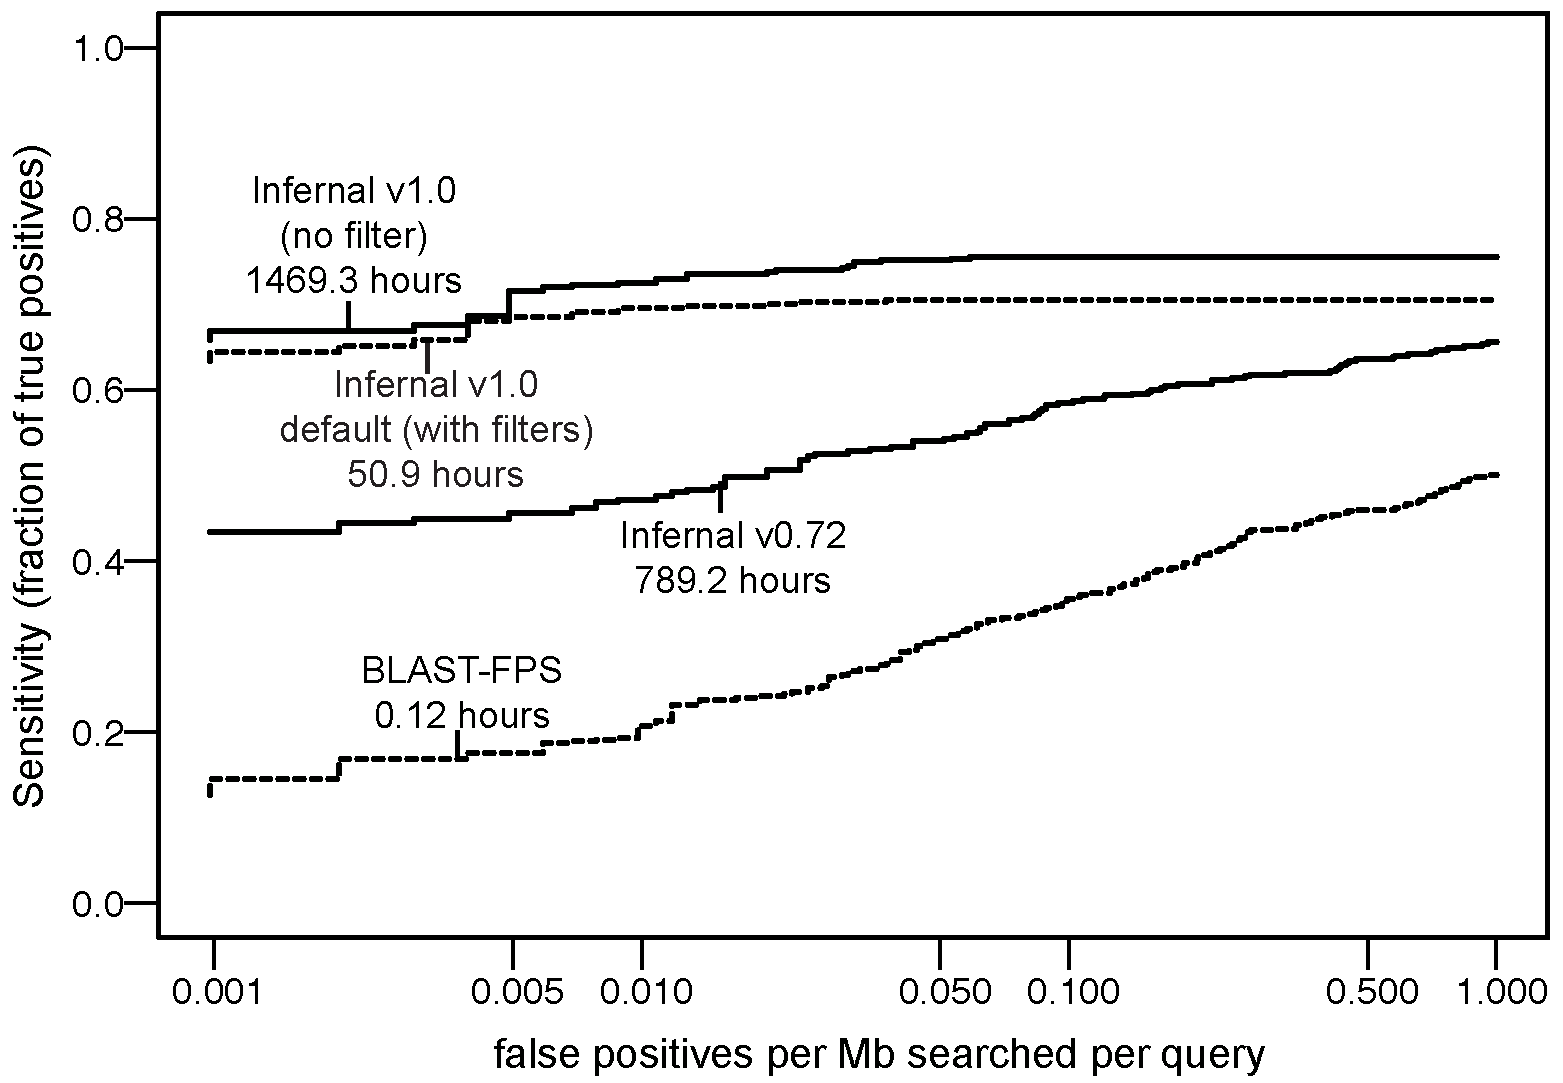
\includegraphics[width=6.4in]{figs/roc}
\caption{\textbf{ROC curves for the benchmark.}  Plots are shown for
the new \textsc{infernal} 1.0 with and without filters, for the old 
\textsc{infernal} 0.72, and for
family-pairwise-searches (FPS) with \textsc{blastn}.}
\label{fig:roc}
\end{center}
\end{figure}

%%%%%%%%%%%%%%%%%%%%%%%%%%%%%%%%%%%%%%%%%%%%%%%%%%%%%%%%%%%%%%%%%%%%%%%
% The 6RNAs table, running times for various applications for 
% 6 RNAs
%\normalfont\ttfamily
\begin{table}[htb]
\begin{center}
\begin{tabular}{lrr|r|rr|r|} 
       & consensus & average \% id   & calibration  & \multicolumn{2}{c|}{search (min/Mb)} & alignment \\
family & length    & in training aln & (hours/model)& no filter & w/filters & (sec/seq) \\ \hline
tRNA    & 71       & 44\%            &       2.8h   &     47.3m &       8.7m&  0.013s \\
5S rRNA & 119      & 56\%            &       2.6h   &     58.6m &      10.1m&  0.026s \\
SRP RNA & 304      & 46\%            &      16.3h   &    333.7m &       5.6m&  0.168s \\
RNaseP  & 365      & 65\%            &      29.9h   &    408.9m &       1.7m&  0.176s \\
SSU rRNA& 1545     & 77\%            &      62.2h   &      n.d. &       n.d.&  1.087s \\
LSU rRNA& 2898     & 82\%            &     134.0h   &      n.d. &       n.d.&  3.072s \\

\end{tabular}

%
% alignment times (a subset of these will be in final table)
% 
% Timings from ~/notebook/8_0909_manuscript_inf-1_appnote/00LOG
% 
% family          & non-banded CYK & HMM banded CYK & HMM banded optacc (default)
%
% tRNA            &       0.049    &         0.0045 &            0.0129
% 5S rRNA         &       0.2023   &         0.0095 &            0.0256
% SRP RNA         &       5.4509   &         0.0615 &            0.1680
% RNase P         &      11.958    &         0.0721 &            0.1759
% SSU rRNA        &     724.201    &         0.7691 &            1.0870
% LSU rRNA        &   11819.9      &         2.5347 &            3.1206
%
%
% search times (a subset of these will be in final table)
% 
% Timings from ~/notebook/8_0909_manuscript_inf-1_appnote/00LOG
% times are per Mb (for forward AND reverse strand) on two input
% seq files: 10Mb.eq.fa   (25% A,C,G,U) = eq
% seq files: 10Mb.real.fa               = reall
% 
%                 ---------------------------------------------------------------------
% family          &    viterbi   &    forward    &     inside       &     filter      &
%                 ---------------------------------------------------------------------
%                 &   eq  & real & eq    & real  &  eq     &  real  &  eq    & real   & 
%                 ---------------------------------------------------------------------
% tRNA            &  6.8s & 6.8s & 20.5s & 20.5s &  2817.2s&  2840.7& 517.8s & 522.1s & 
% 5S rRNA         & 10.1s &10.0s & 32.1s & 32.0s &  3516.3 &  3517.5& 612.9s & 607.5s & 
% SRP RNA         & 22.6s &22.6s & 77.1s & 77.2s & 20099.3 & 20024.0& 878.9  & 335.3s &
% RNase P         & 26.9s &26.9s & 94.1s & 94.2s & 24533.3 & 24559.9& 124.1  & 103.3s &
% SSU rRNA        & 
% LSU rRNA        & 
%
\end{center}
\caption{\textbf{Calibration, search, and alignment running times for
    six known structural RNAs of various sizes.} SSU rRNA and LSU rRNA
    search times were not determined (n.d.) because faster non-CM
    methods are well suited for finding these RNAs due to their high
    level of primary sequence conservation.  . }
\label{tbl:times}
\end{table}

\newpage
%\bibliography{distilled}
\bibliography{master,books,lab}

\end{document}

\section{Acknowledgements}

\section{Funding}
EPN and SRE are supported by Howard Hughes Medical Institute.

%%%%%%%%%%%%%%%%%%%%%%%%%%%%%%%%%%%%%%%%%%%%%%%%%%%%%%%%%%%
%%%%%%%%%%%%%%%%%%%%%%%%%%%%%%%%%%%%%%%%%%%%%%%%%%%%%%%%%%%
%%%%%%%%%%%%%%%%%%%%%%%%%%%%%%%%%%%%%%%%%%%%%%%%%%%%%%%%%%%

%%%%%%%%%%%%%%%%%%%%%%%%%%%%%%%%%%%%%%%%%%%%%%%%%%%%%%%%%%%
% OTHER POSSIBLE TABLES/FIGURES
%
% kept here for convenience in case they're needed later
%%%%%%%%%%%%%%%%%%%%%%%%%%%%%%%%%%%%%%%%%%%%%%%%%%%%%%%%%%%

%%%%%%%%%%%%%%%%%%%%%%%%%%%%%%%%%%%%%%%%%%%%%%%%%%%%%%%%%%%%%%%%%%%%%%%
% GC content figure 
%
\begin{comment}
\begin{figure}
\begin{center}
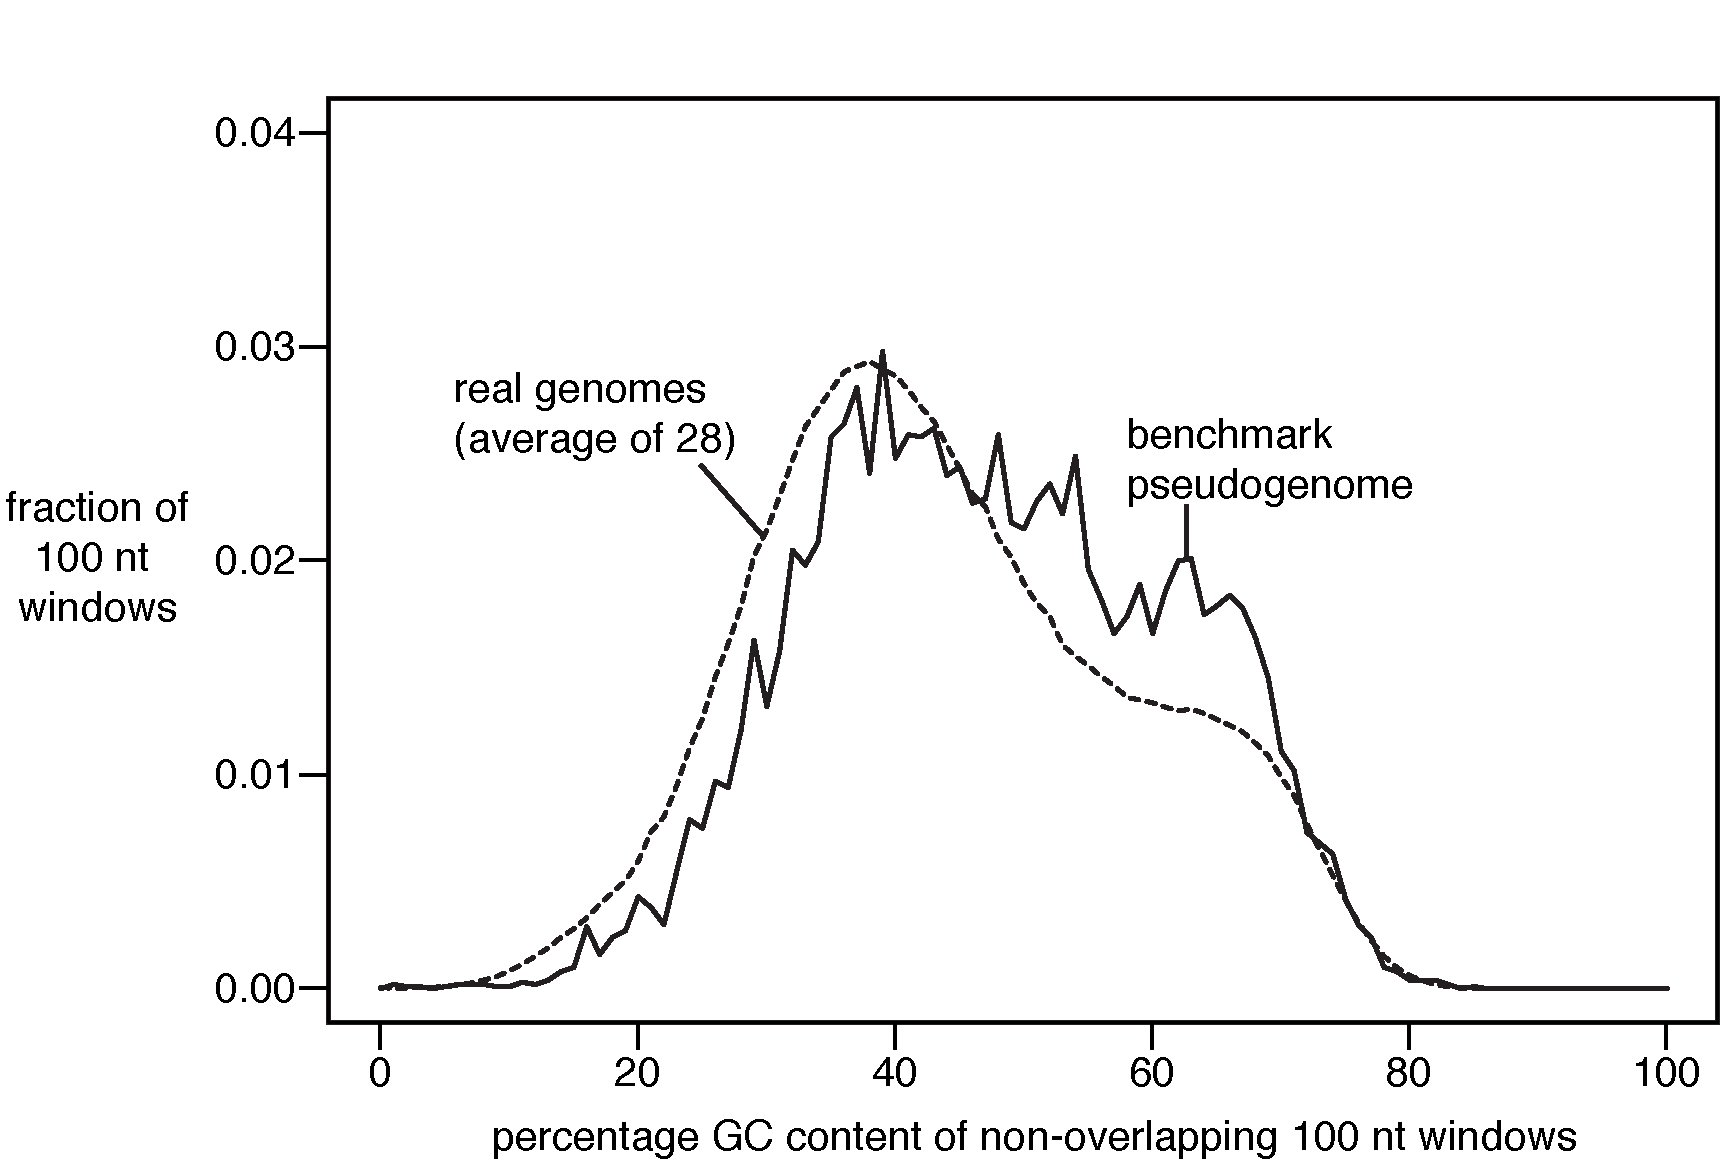
\includegraphics[width=6.4in]{figs/gc}
\caption{\textbf{GC content of 100 nucleotide windows in the
    benchmark pseudogenome and in a sampling of real genomic segments.}}  
\label{fig:gc-realmark}
\end{center}
\end{figure}
\end{comment}
%%%%%%%%%%%%%%%%%%%%%%%%%%%%%%%%%%%%%%%%%%%%%%%%%%%%%%%%%%%%%%%%%%%%%%%
% 6 RNAs table, different formatted
\begin{comment}
\begin{table}[htb]
\begin{center}
\begin{tabular}{ccccccr} 

       & consensus & \multicolumn{3}{c}{homology search} &  & alignment \\ \hline
family & length    & hmm & cm    & filtered & calibration   & sec/seq   \\ \hline
%                    fwd   inside non-banded
tRNA    & 71       & 20.5s & 3030s  & 522.1s   & 2.8h        & 0.013 \\
5S rRNA & 119      & 32.1s & 2941s  & 607.5s   & 2.6h        & 0.026 \\
SRP RNA & 304      & 77.2s & 25000s & 335.3s   & 16.3h       & 0.168 \\
RNaseP  & 365      & 94.1s & 50000s & 103.3s   & 29.9h       & 0.176 \\
SSU rRNA& 1545     &  ?    & ?      & ?        & 62.2h       & 1.087 \\
LSU rRNA& 2898     &  ?    & ?      & ?        & 134.0h      & 3.072 \\
\end{tabular}
\end{comment}
%%%%%%%%%%%%%%%%%%%%%%%%%%%%%%%%%%%%%%%%%%%%%%%%%%%%%%%%%%%%%%%%%%%%%%
% The rmark MER table - summary MERs
%\normalfont\ttfamily
\begin{comment}
\begin{table}[htb]
\begin{center}

\begin{tabular}{lccr} 

program & MER & hours \\ \hline
\textsc{blastn}                    & 286 &   0.02 \\
\textsc{infernal} 0.55             & 234 & 564.9  \\
\textsc{infernal} 0.72             & 185 &  84.0  \\
\textsc{infernal} 1.0 non-filtered & 109 & 159.0  \\
\textsc{infernal} 1.0 default      & 124 &  12.6  \\

\begin{tabular}{lccr} 

        & \multicolumn{2}{c}{MER} & \\
program & non-biased & biased & hours \\ \hline

\textsc{blastn}                    & 216 & 286 &   0.02 \\
\textsc{infernal} 0.55             & 232 & 234 & 564.9  \\
\textsc{infernal} 0.72             & 114 & 185 &  84.0  \\
\textsc{infernal} 1.0 non-filtered & 109 & 109 & 159.0  \\
\textsc{infernal} 1.0 default      & 120 & 124 &  12.6  \\

\end{tabular}
\end{center}
\caption{\textbf{Rfam benchmark MER summary statistics.}} 
\label{tbl:rmarkmerlist}
\end{table}
\end{comment}
%%%%%%%%%%%%%%%%%%%%%%%%%%%%%%%%%%%%%%%%%%%%%%%%%%%%%%%%%%%%%%%%%%%%%%%




